\documentclass{standalone}
\usepackage{xcolor}
\usepackage{verbatim}
\usepackage[T1]{fontenc}
\usepackage{graphics}
\usepackage{hyperref}
\newcommand{\code}[1]{\texttt{#1}}
\newcommand{\R}{R}
\newcommand{\pkg}[1]{#1}
\newcommand{\CRANpkg}[1]{\pkg{#1}}%
\newcommand{\BIOpkg}[1]{\pkg{#1}}
\usepackage{amsmath,amssymb,array}
\usepackage{booktabs}
\usepackage{multicol, calc}
\usepackage{tikz}
\usetikzlibrary{patterns,positioning,babel}
\usepackage{threeparttable}
\usepackage{natbib}
\usepackage{inconsolata}
\usepackage{listings}
\usepackage{tikz-qtree}
\usepackage{subcaption} 

\begin{document}
\nopagecolor
	
		
		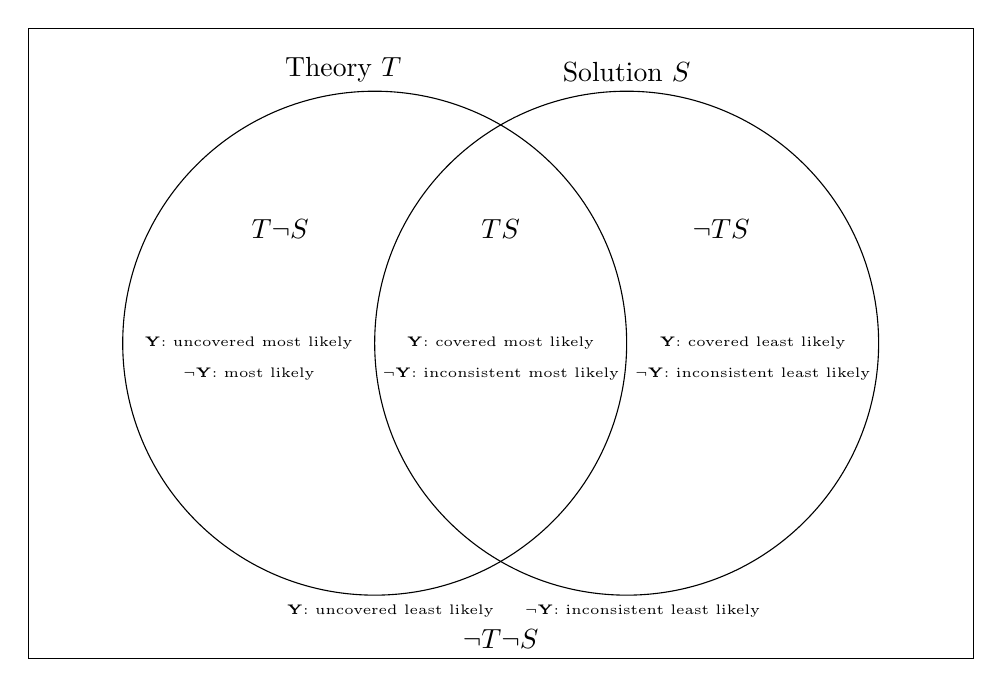
\begin{tikzpicture}[scale=4]
		\draw (0,0) rectangle (3,2);
		\draw (1.1,1) circle [radius=0.8];
		\node[above] at (1,1.8) {Theory $T$};
		\draw (1.9,1) circle [radius=0.8];
		\node[above] at (1.9,1.8) {Solution $S$};
		\node[above] at (0.8,1.3) {\textbf{$T \neg S$}};
		\node[above] at (1.5,1.3) {\textbf{$TS$}};
		\node[above] at (1.5,0) {\textbf{$\neg T \neg S$}};
		\node[above] at (2.2,1.3) {\textbf{$\neg TS$}};
		\node[above] at (0.7,0.95) {\tiny \textbf{Y}: uncovered most likely};
		\node[above] at (0.7,0.85) {\tiny \textbf{$\neg$Y}: most likely};
		\node[above] at (1.5,0.95) {\tiny \textbf{Y}: covered most likely};
		\node[above] at (1.5,0.85) {\tiny \textbf{$\neg$Y}: inconsistent most likely};
		\node[above] at (2.3,0.95) {\tiny \textbf{Y}: covered least likely};
		\node[above] at (2.3,0.85) {\tiny \textbf{$\neg$Y}: inconsistent least
			 likely};
		\node[above] at (1.15,0.1) {\tiny \textbf{Y}: uncovered least likely};
		\node[above] at (1.95,0.1) {\tiny \textbf{$\neg$Y}: inconsistent least likely};
		\end{tikzpicture}
\end{document}
